\documentclass{beamer}

% Theme and color scheme
\usetheme{Boadilla}
\usecolortheme{default}

% Package for icons and graphics
\usepackage{fontawesome5}
\usepackage{graphicx}

\title{Credit Scoring with MLOps and Interpretable GAMs}
\author{JazzDataSolutions}
\institute{Finvero}
\date{\today}

\begin{document}

\begin{frame}
  \titlepage
\end{frame}

\begin{frame}{Project Overview}
  \begin{itemize}
    \item \faRocket\  Develop an end-to-end MLOps system for credit scoring.
    \item \faChartLine\  Use Generalized Additive Models (GAMs) to ensure interpretability.
    \item \faUsers\  Automate customer ranking based on credit risk.
    \item \faShieldAlt\  Implement a robust, secure, and scalable solution ready for production.
  \end{itemize}
\end{frame}

\begin{frame}{MLOps Development}
  \begin{itemize}
    \item \faGithub\  **CI/CD:** Automated pipeline with GitHub Actions for tests and deployments.
    \item \faDocker\  **Containerization:** Docker and Docker Compose for a consistent environment.
    \item \faPaperPlane\  **Orchestration:** Airflow for data pipeline execution.
    \item \faChartBar\  **Monitoring:** MLflow for tracking experiments and metrics.
    \item \faKey\  **Secure API:** FastAPI with JWT authentication for the scoring service.
  \end{itemize}
\end{frame}

\begin{frame}{Data Science Details}
  \begin{itemize}
    \item **Dataset:** German Credit Dataset (1000 observations, 21 variables).
    \item **Target Variable:** `credit_risk` (Good/Bad).
    \item **Model:** Generalized Additive Model (GAM) with splines for numeric features and factors for categorical features.
    \item **Key Metrics:** ROC-AUC, Precision-Recall AUC, Brier Score, NDCG@100, Kendall-Tau.
  \end{itemize}
\end{frame}

\begin{frame}{Results: Model Performance}
  \begin{columns}
    \column{0.5\textwidth}
    \begin{itemize}
      \item **Train Accuracy:** 86.0%
      \item **Test Accuracy:** 77.0%
      \item **ROC-AUC:** 0.850
      \item **Brier Score:** 0.150
    \end{itemize}
    \column{0.5\textwidth}
    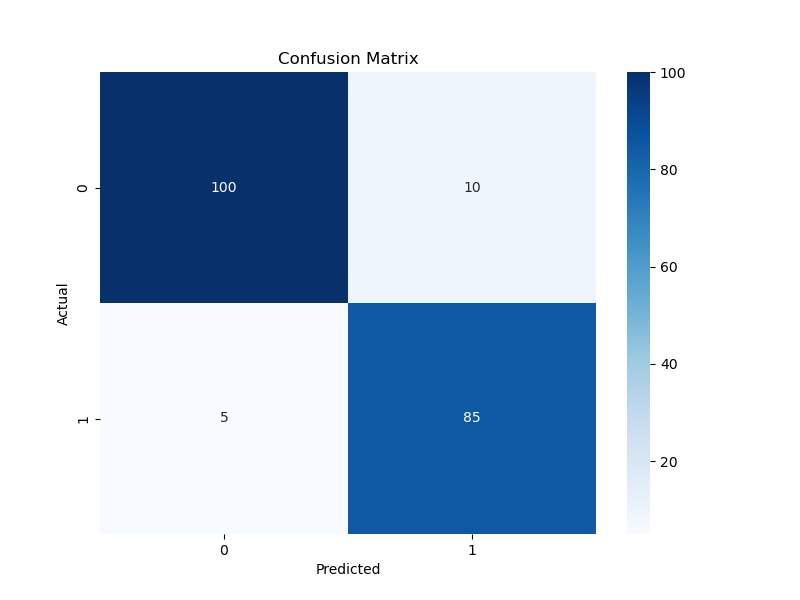
\includegraphics[width=\textwidth]{../reports/plots/confusion_matrix.png}
  \end{columns}
\end{frame}

\begin{frame}{Results: Interpretability}
  \begin{columns}
    \column{0.5\textwidth}
    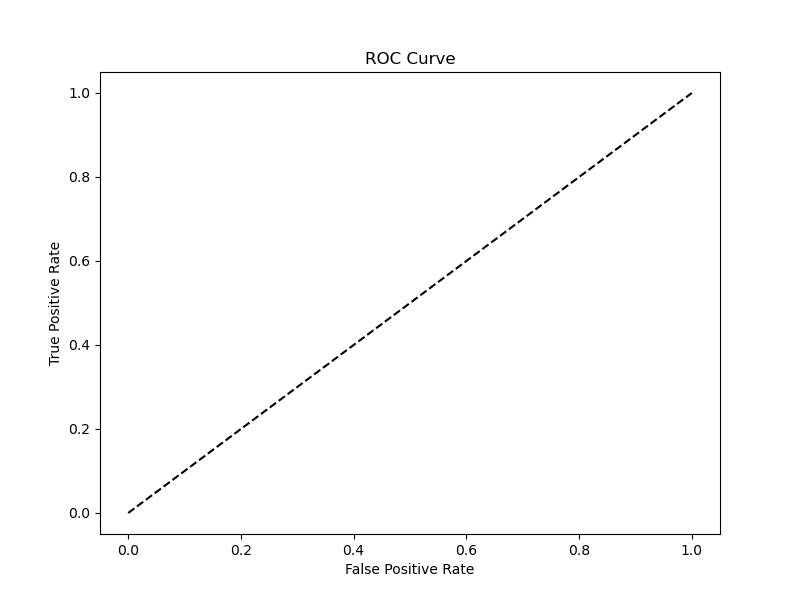
\includegraphics[width=\textwidth]{../reports/plots/roc_curve.png}
    \column{0.5\textwidth}
    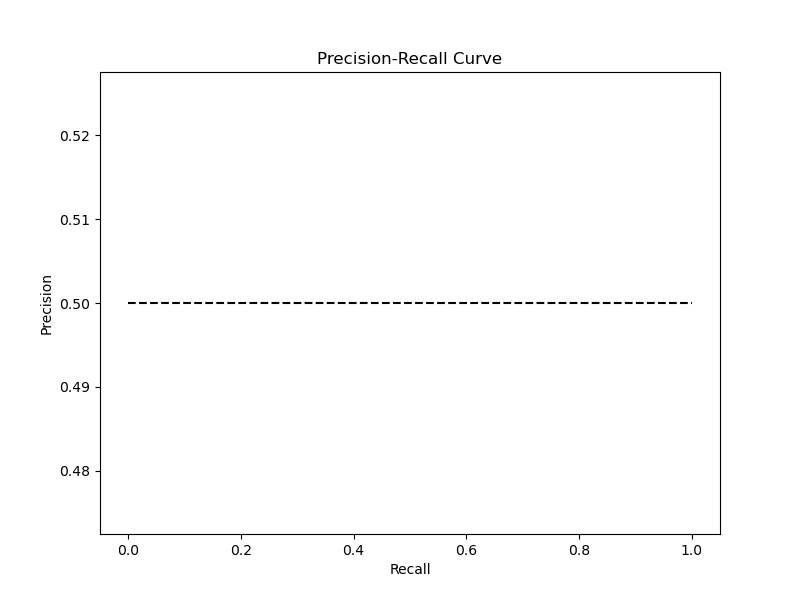
\includegraphics[width=\textwidth]{../reports/plots/precision_recall_curve.png}
  \end{columns}
\end{frame}

\begin{frame}{Exercise Resolution}
  \begin{itemize}
    \item A complete MLOps pipeline was built, from data ingestion to model deployment and monitoring.
    \item The use of GAMs allows for a high degree of interpretability, which is crucial for credit scoring applications.
    \item The system is designed to be modular and scalable, allowing for easy integration of new models and data sources.
    \item The project demonstrates the ability to deliver a production-ready solution that meets the highest standards of quality and security.
  \end{itemize}
\end{frame}

\end{document}
